\chapter{Introduction}
%labels will help you to reference to certain images, tables, chapters, section, and so on...
\label{introduction}
%DELETEME: for readability purpose, it makes sense to write a short paragraph on what the reader can expect in this chapter.
%
%DELETEME: tipp: sometimes it makes sense to write the first chapter, the last chapter, and the abstracts at the end. In this case, it might be easier to argue towards your topic
\textcolor{magenta}{talk about approaches (retrieval-based models / using ML / NLP...), modularization and Einteilung of the paper}


%###################################################################################
%###################### Motivation          ########################################
%###################################################################################
\section{Motivation}

%DELETEME: This section is very important since it argues why it is necessary to take care of the problem you are addressing in your work. One way to do this is coming from a very broad view on the problem to a very detailled one. This can be done by establishing a chain of statements that refer to each other until you reach your particular problem. Doing this, you really need to take care for citing every statement.

%DELETEME: Example for a chain: Mobile communication gets increasingly popular in the world (CITE sales on mobile communication infrastruce, mobile phones, or increasing number of mobile phones contracts). $\rightarrow$ Especially smartphones, which represent the next generation cellular phone (CITE), get more and more used for communicating not only with other people but also for connecting to the Internet for using various services (CITE). $\rightarrow$ Smartphone are comprehensive cellular phones that provide additional functionality due to their increased connection and processing capabilities (CITE). $\rightarrow$ Most smartphones offer an online application store for adding software to the devices which helps the users to customize their devices according to their needs, e.g. Android Market\footnote{\url{http://market.android.com}, visited on 05/08/2011}. $\rightarrow$ One problem about installing third-party software is that not all softwares try to help the user; $\rightarrow$ software with malicious intentions, so called malicious software (malware), can be a severe threat to smarpthone users. Some malwares delete files (EXAMPLE + CITE or footnote with URL) or even destroy devices (EXAMPLE + CITE or footnote with URL). $\rightarrow$ More and more smartphone malwares appeared in the last years (CITE). $\rightarrow$ Signature-based approaches work efficiently on known malware (CITE) but face serious drawbacks regarding unknown malware. $\rightarrow$ Oberheide et al.~\cite{oberheide:2008:cloudav} state that virus engines need an average time of 48 days until their databases get updated to be able to detect a certain unknown malware. $\rightarrow$ This in turn means that smartphone users stay unprotected for this time which can be seen as a severe threat. $\rightarrow$ Therefore, approaches are needed that are capable of detecting unknown malware for protecting the users against such threats.
%DELETEME: This example showed how one could argue that alternative approaches for malware detection is required. The length of the motivation depends on the topics handled and can of course be longer. The principle I am describing is also shown on Figure~\ref{fig:writing}

Human interaction with machines on an advanced level has always been an aspiration of the future. With evidence in fiction readings Sci-Fi films \textcolor{magenta}{citation}, societies have shown an increasing tendency to avail technologies that make computers present in most domains of our daily lives. And though we still are far from it, we have come a long way in the recent years. With the boom of artificial intelligence and devices making high processing power a tangible option \textcolor{magenta}{statistic from graph about messenger surpassing social networks - Screen Shot 2017-11-19 at 17.15.18}
\textcolor{magenta}{More and more people "trust" new technologies and the trends resulting from there, be it social media, alexa, selfies and no.. ripple effect - More use 'hey Siri' -> results of data collected, what we know about people more than ever before}

\subsection{history of bots}
\textcolor{magenta}{
- then: eliza psychoanalyzer\\
- now: Xiaoice: empathetic bot in china\\
}
\subsection{Why Bots?}
\textcolor{magenta}{
- den menschlichen Aspekt suggerieren\cite{hiddenbrainpod}\\
- menschliches Verhalten immitieren\\
- smalltalk f\"ahigkeiten\\
- imagination about ablitiy to react to everything\\
- how these are centralized at alexa somewhere ->> SKILLS, amazon.com\\
- what are classic use cases for their use with prominent examples? Booking tickets (KLM bot),\\
- \href{https://www.forbes.com/sites/tomaslaurinavicius/2017/04/24/facebook-messenger-bots/\#4f61c16a66d8}{fun bots} and more
- unfortunately forums and FAQ pages are not as effective as talking to a human.\\ 
a- then again, as a customer, if i want assistance, I want the customer to tell me a model number etc.}
\subsection{Can they replace humans?}
Although not impossible, it is a bit too far-fetched at this stage.\\
\textcolor{magenta}{
%	- mention development from metager / altavista to google. what u do with facets vs an all in predictor - we are at a stage where bots are like altavista..u tell alexa to open a skill like u tell altavista to look in pics or go to lexisnexis to do reserach. we are yet to reach the state of watson like google is to searches
-	Difference between bot and human in response\\
human says long sentences and there is a fluid transition between dialog and monologue 
-con: the bot wants a sentence yesharra7a f 7etat soghayara w neshouf..nicht unendlich lang\\
- otherwise, error margin too large.\\
- this has to do with human language complexity.\\
Why can't robots understand us\\
- language is ambiguous, we need to understand context\\
--Syntactical: Homonyme\\ %fly, fly,  presently I’ll present you a present - now, give, gift
--Semantic:  Methaphors, %“it’s raining cats and dogs”
sarcasm, %“oh yea, sounds very exciting”
and puns\\
\\
--dialects: enunciations\\
--underlying grammar\\ %“what makes you abcd just now
--underlying sentiment\\
\\
-progress in NLP making bots great again\\
-neural networks: help understanding language patterns and get better over time\\
thought vectors: helps connect different words with related meaingns\\
\\
chatbots as enablers in customer service industry\\
reply suggestions function - with the aforementioned techniques, such functionality becomes possible\\
\\
- it would speak as an advantage for bots if they can determine these things automatically z.B.\\
- besides, I could be a bit more sure in customer support scenario that a bot won't trick me\\
- as a novice I am usually not sure if the help article / Kbase I am reading is the right one\\
- and forums have mostly Schrott anyway.\\
- what bots already achieved is at least not to give wrong answers.\\
- they could sometimes say idk, which is annoying, but at least it doesn't confuse the user.\\
- next step is to get around the user's frustration by making the bot at least more human.
}


\subsection{Topology of Bots}
\textcolor{magenta}{
-use cases and purpose categories (leisure, productivity) - quick survey of respective 'AppStores'
-\href{https://www.npr.org/podcasts/510308/hidden-brain}{platforms}
-physical locations (home, office, car, phone, in a business)
}

\subsection{Information bots}
\textcolor{magenta}{
	- mention available service types (information system as a "webpage/database")\\
	- vs an interactive bot that gives you customized information on demand
	hier soll der D115 Anwendungsfall "Beauskunftung" kurz erl\"autert werden\\
}
\subsection{social bots}
\textcolor{magenta}{
	- with advantages / disadvantages\\
	- fake news / online reviews\\
}

\subsection{bot-type}
\textcolor{magenta}{
- use of ML
Handyversicherungsbeispiel\\
- from business perspective, the bot is aiming to sell more polices,\\ 
- the bot tries to determine if there is a nuance in the user's answer (machine acting as a judge!)
- e.g. ``how did the phone fall off``
- MKTG - Aufwand
}
%\begin{figure}
%\centering
%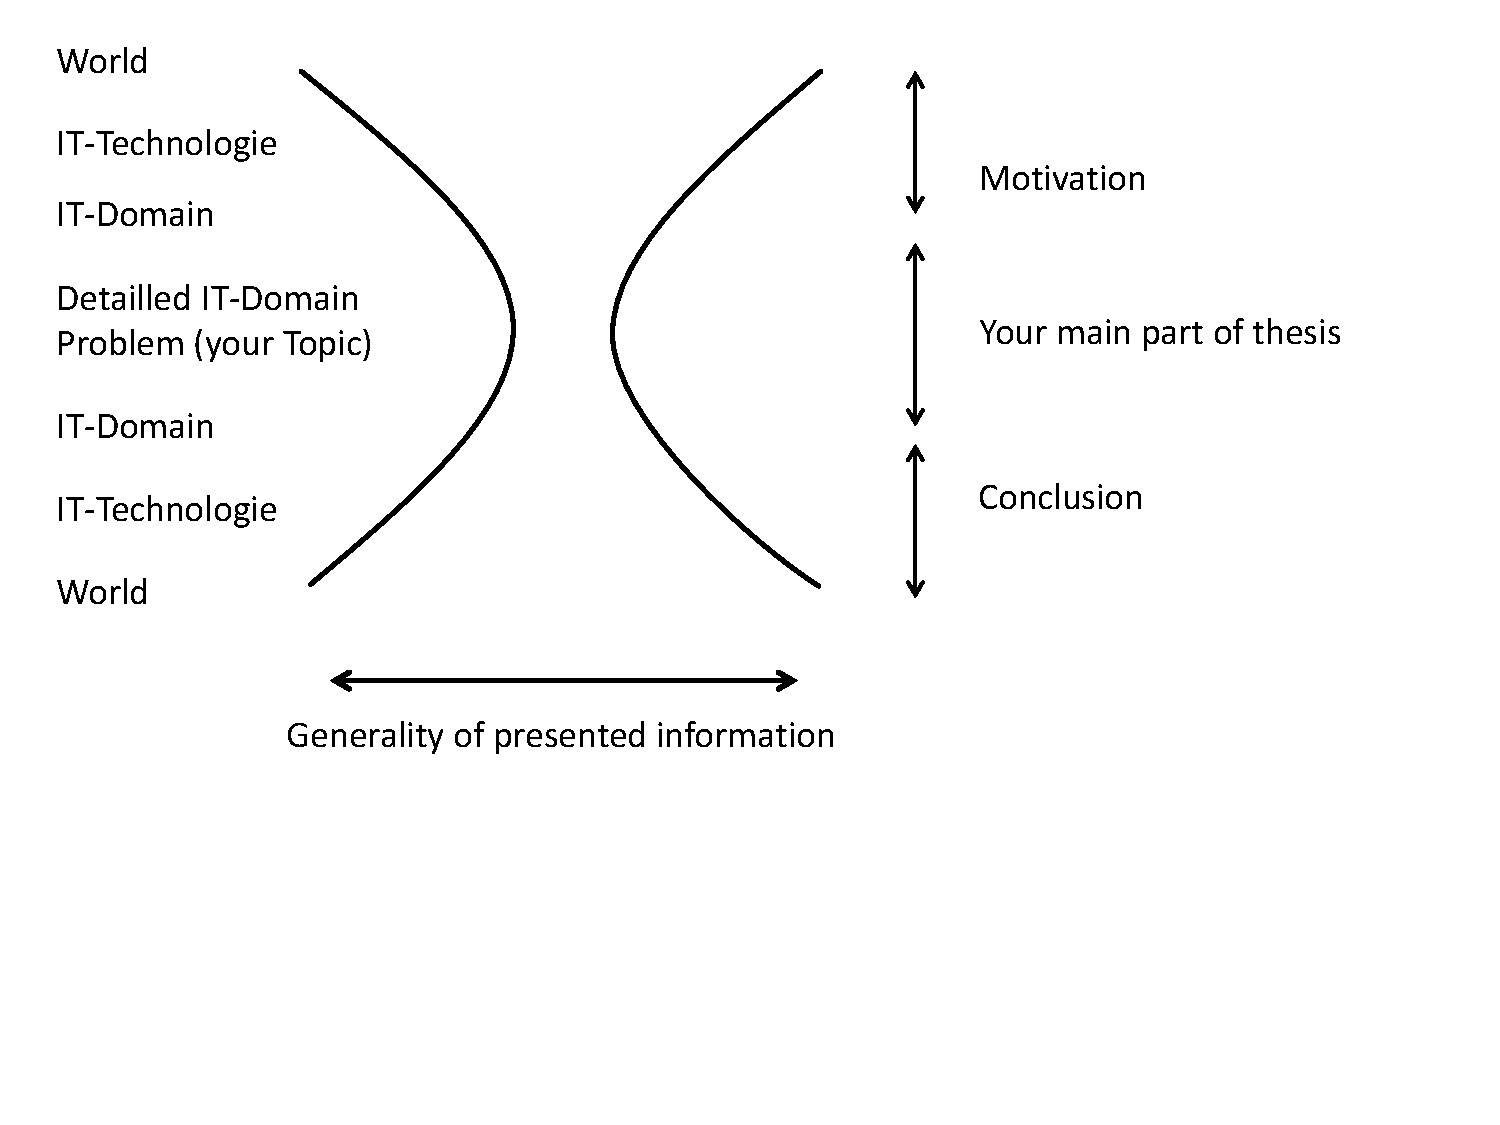
\includegraphics[width=0.9\textwidth]{template/writing}
%\caption[Information Generality]{This images illustrates how generality of information could be handled in a thesis. In your motivation you should start from a very broad view on the topic. Then you should get more precise with every statement until you reach the actual problem you are addressing. You should do vice-versa in your conclusion, starting with the problem that you addressed and getting broader until you can write about the meaning of your results to the (IT-)world.\label{fig:writing}}
%\end{figure}





%###################################################################################
%###################### State of the Art  ########################################
%###################################################################################
\section{State of the Art}

\subsection{API.ai}

\subsection{Facebook Messenger Chatbots}
\subsection{wit.ai}
\subsection{motion.ai}

\subsection{Alexa Skills}
\subsection{Amazon Voice Service}

\subsection{Amazon Lex}

%###################################################################################
%###################### Approach and Goals  ########################################
%###################################################################################
\section{Approach and Goals}
%DELETEME: In this section, you should cleary describe your approach that you are following in order to solve the underlaying problem of your thesis. Additionally, you should clearly state the goals of your work. This will not only help you supervizor to understand what you are doing, it will also help you to be sure on which topic you should evaluate.
\textcolor{magenta}{
	- making the bot become something beyond a Q\&A:\\
	- \href{https://www.youtube.com/watch?v=QxgdPI1B7rg}{Alexa Documentation}\\
	- retaining sessions (explain requests/responses - GET/POST)\\
	- fullfilling intents\\
	- nested handlers\\
	\\
	- for facebook: implementing the three-answer suggestions\\
	\\
	- internationalization / customization based on Locale
	- why is it important?\\
	- many international users prefer a chatbot than a phone since the bot will commmunicate more accurately, will not have language probs if it understands the foreign lang etc.\\
	- what are other approaches to localization? refer to IRS lecture notes\\
	- use of translators, Stammsprache, etc., detecting the language and say it does not support it.\\ 
	\\
	- Alexa Skill will work in germany in english and german -> add english after german\\
	-AL: Anschlie{\ss}end soll das Ziel der Arbeit formuliert werden: Entwicklung und Evaluation eines Prototypen f\"ur den Anwendungsfall.\\
}

%###################################################################################
%###################### Structure of the Thesis ####################################
%###################################################################################
\section{Structure of the Thesis}
%DELETEME: This section does not require eloquent writing. It is just a presentation of what you will handle in each chapter starting with Chapter~\ref{background}.
%
%DELETEME: Example: This thesis is structured as follows. In Chapter~\ref{background}, we discuss essential background related to the thesis topic. (SOME MORE SENTENCES). Chapter~\ref{mainone} represents a detailled analysis of the problem that will be addressed. In particular, (SOME MORE SENTENCES). In Chapter~\ref{maintwo}, our solution is presented. This solution covers ... (SOME MORE SENTENCES). Chapter~\ref{evaluation} evaluates our solution basing on our specified goals. (SOME MORE SENTENCES). In Chapter~\ref{conclusion}, we conclude. Chapter~\ref{appendices} gives additional related information on the topic of this thesis.